% Created by tikzDevice version 0.8.1 on 2015-06-30 12:22:41
% !TEX encoding = UTF-8 Unicode
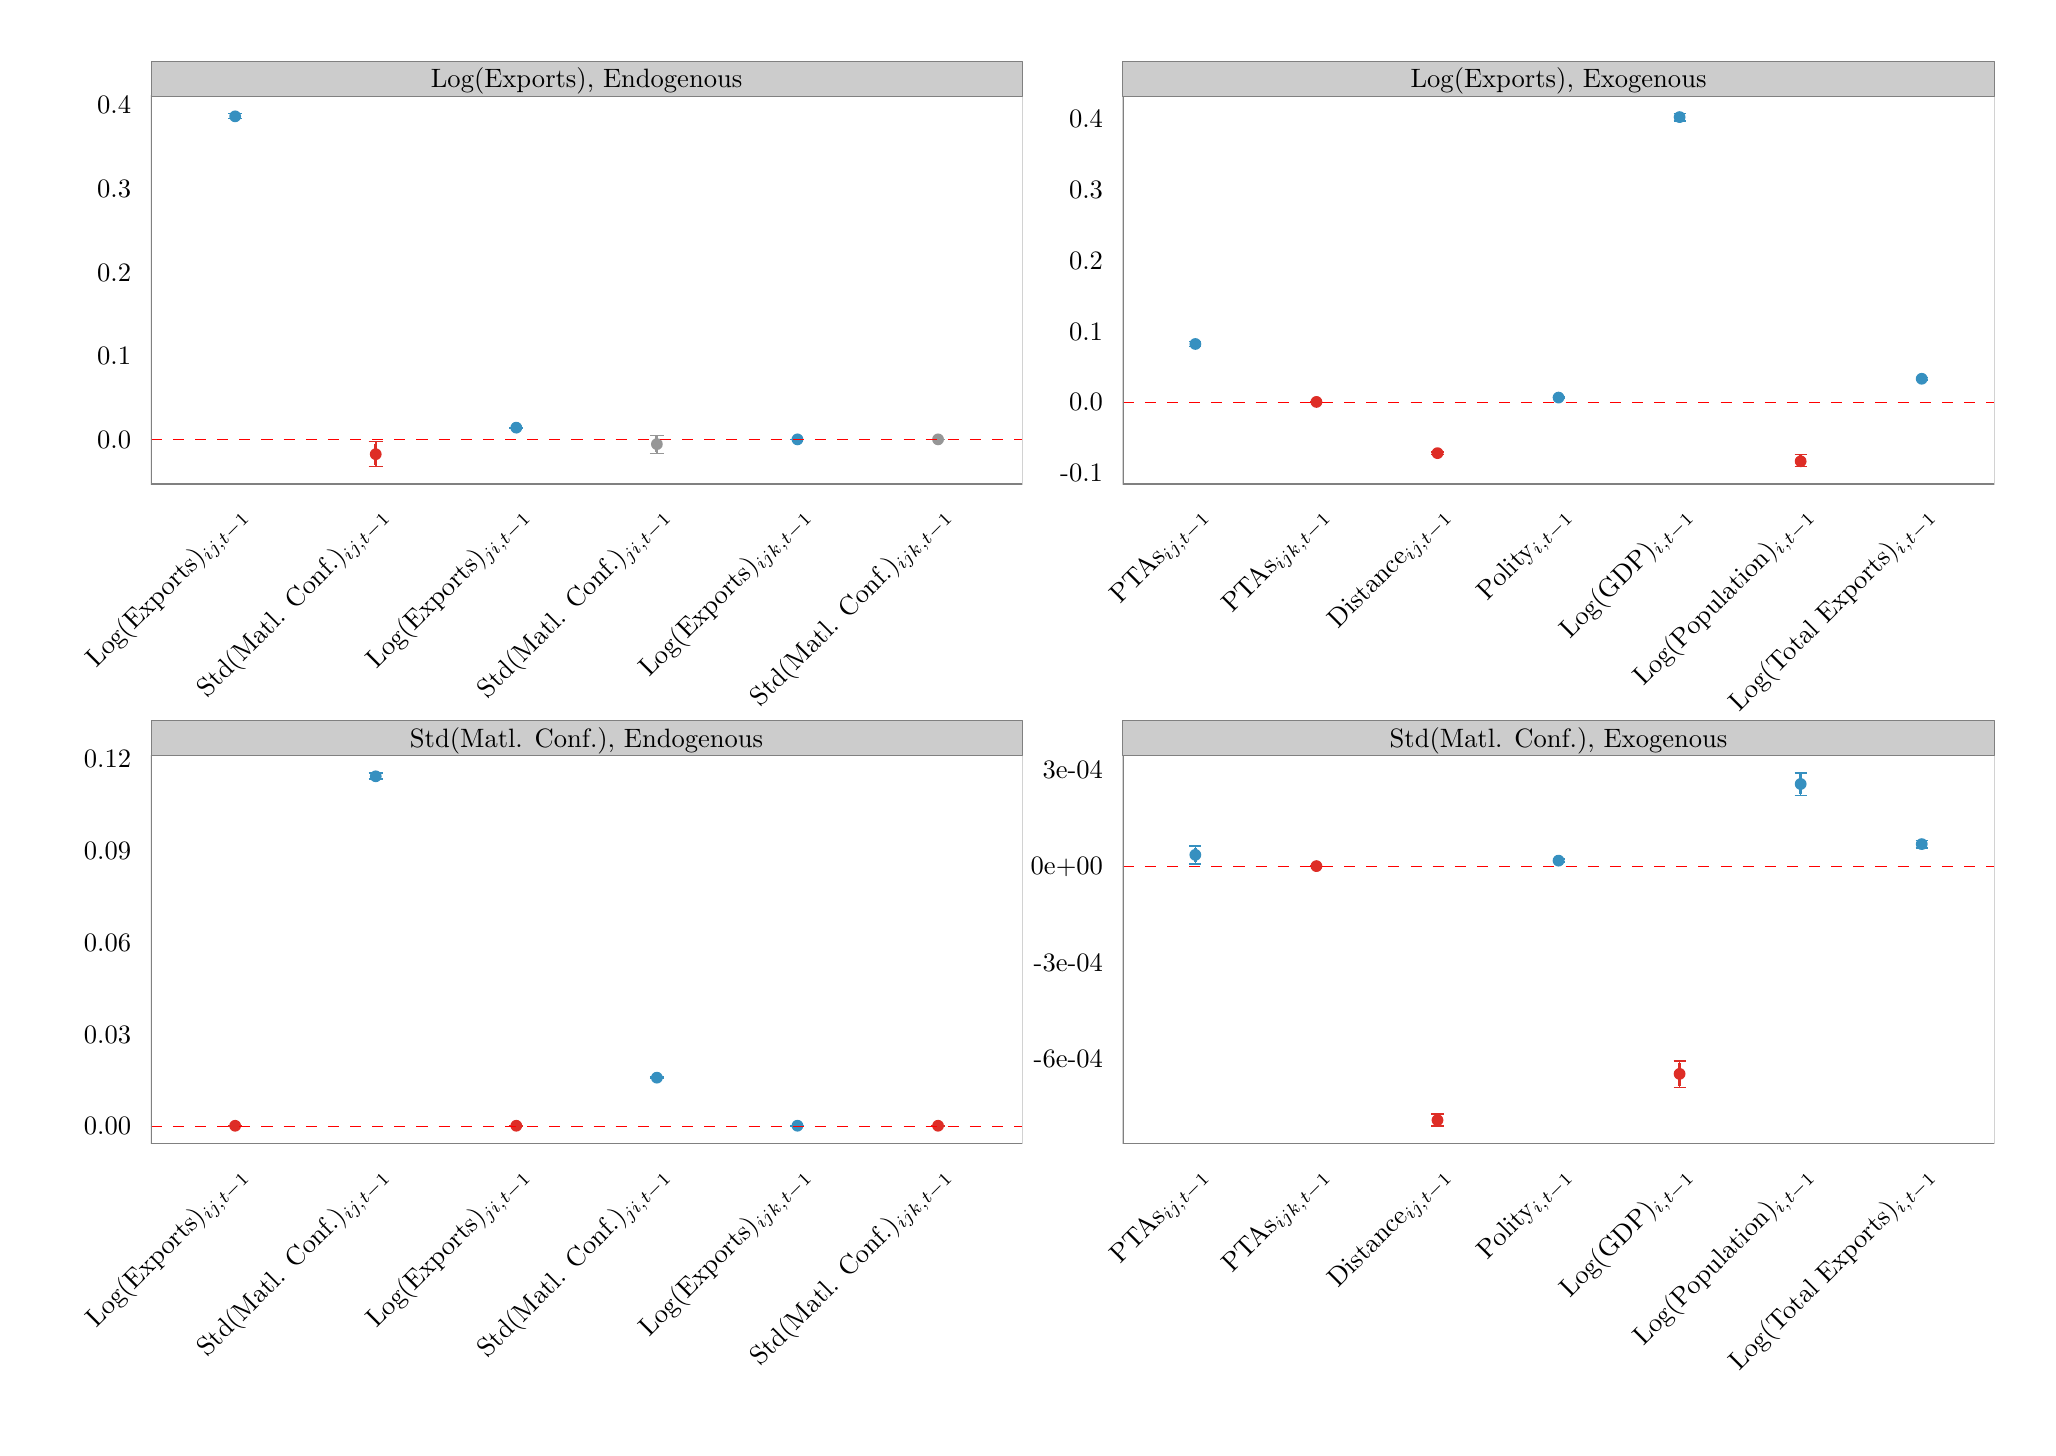
\begin{tikzpicture}[x=1pt,y=1pt]
\definecolor{fillColor}{RGB}{255,255,255}
\path[use as bounding box,fill=fillColor,fill opacity=0.00] (0,0) rectangle (722.70,505.89);
\begin{scope}
\path[clip] (  0.00,  0.00) rectangle (722.70,505.89);
\definecolor{drawColor}{RGB}{255,255,255}
\definecolor{fillColor}{RGB}{255,255,255}

\path[draw=drawColor,line width= 0.6pt,line join=round,line cap=round,fill=fillColor] (  0.00,  0.00) rectangle (722.70,505.89);
\end{scope}
\begin{scope}
\path[clip] ( 44.49,340.99) rectangle (359.44,481.21);
\definecolor{fillColor}{RGB}{54,144,192}

\path[fill=fillColor] ( 74.97,473.84) circle (  2.13);
\definecolor{fillColor}{RGB}{222,45,38}

\path[fill=fillColor] (125.77,351.76) circle (  2.13);
\definecolor{fillColor}{RGB}{54,144,192}

\path[fill=fillColor] (176.56,361.35) circle (  2.13);
\definecolor{fillColor}{gray}{0.59}

\path[fill=fillColor] (227.36,355.40) circle (  2.13);
\definecolor{fillColor}{RGB}{54,144,192}

\path[fill=fillColor] (278.16,357.12) circle (  2.13);
\definecolor{fillColor}{gray}{0.59}

\path[fill=fillColor] (328.96,357.12) circle (  2.13);
\definecolor{drawColor}{RGB}{54,144,192}

\path[draw=drawColor,draw opacity=0.30,line width= 0.3pt,line join=round] ( 74.97,473.08) -- ( 74.97,474.84);
\definecolor{drawColor}{RGB}{222,45,38}

\path[draw=drawColor,draw opacity=0.30,line width= 0.3pt,line join=round] (125.77,347.36) -- (125.77,356.34);
\definecolor{drawColor}{RGB}{54,144,192}

\path[draw=drawColor,draw opacity=0.30,line width= 0.3pt,line join=round] (176.56,361.24) -- (176.56,361.45);
\definecolor{drawColor}{RGB}{150,150,150}

\path[draw=drawColor,draw opacity=0.30,line width= 0.3pt,line join=round] (227.36,352.03) -- (227.36,358.57);
\definecolor{drawColor}{RGB}{54,144,192}

\path[draw=drawColor,draw opacity=0.30,line width= 0.3pt,line join=round] (278.16,357.12) -- (278.16,357.12);
\definecolor{drawColor}{RGB}{150,150,150}

\path[draw=drawColor,draw opacity=0.30,line width= 0.3pt,line join=round] (328.96,357.11) -- (328.96,357.13);
\definecolor{drawColor}{RGB}{54,144,192}

\path[draw=drawColor,line width= 1.1pt,line join=round] ( 74.97,473.15) -- ( 74.97,474.72);
\definecolor{drawColor}{RGB}{222,45,38}

\path[draw=drawColor,line width= 1.1pt,line join=round] (125.77,347.92) -- (125.77,355.59);
\definecolor{drawColor}{RGB}{54,144,192}

\path[draw=drawColor,line width= 1.1pt,line join=round] (176.56,361.27) -- (176.56,361.44);
\definecolor{drawColor}{gray}{0.59}

\path[draw=drawColor,line width= 1.1pt,line join=round] (227.36,352.66) -- (227.36,358.16);
\definecolor{drawColor}{RGB}{54,144,192}

\path[draw=drawColor,line width= 1.1pt,line join=round] (278.16,357.12) -- (278.16,357.12);
\definecolor{drawColor}{gray}{0.59}

\path[draw=drawColor,line width= 1.1pt,line join=round] (328.96,357.11) -- (328.96,357.13);
\definecolor{drawColor}{RGB}{54,144,192}

\path[draw=drawColor,line width= 0.6pt,line join=round] ( 72.43,474.84) --
	( 77.51,474.84);

\path[draw=drawColor,line width= 0.6pt,line join=round] ( 74.97,474.84) --
	( 74.97,473.08);

\path[draw=drawColor,line width= 0.6pt,line join=round] ( 72.43,473.08) --
	( 77.51,473.08);
\definecolor{drawColor}{RGB}{222,45,38}

\path[draw=drawColor,line width= 0.6pt,line join=round] (123.23,356.34) --
	(128.31,356.34);

\path[draw=drawColor,line width= 0.6pt,line join=round] (125.77,356.34) --
	(125.77,347.36);

\path[draw=drawColor,line width= 0.6pt,line join=round] (123.23,347.36) --
	(128.31,347.36);
\definecolor{drawColor}{RGB}{54,144,192}

\path[draw=drawColor,line width= 0.6pt,line join=round] (174.03,361.45) --
	(179.10,361.45);

\path[draw=drawColor,line width= 0.6pt,line join=round] (176.56,361.45) --
	(176.56,361.24);

\path[draw=drawColor,line width= 0.6pt,line join=round] (174.03,361.24) --
	(179.10,361.24);
\definecolor{drawColor}{gray}{0.59}

\path[draw=drawColor,line width= 0.6pt,line join=round] (224.82,358.57) --
	(229.90,358.57);

\path[draw=drawColor,line width= 0.6pt,line join=round] (227.36,358.57) --
	(227.36,352.03);

\path[draw=drawColor,line width= 0.6pt,line join=round] (224.82,352.03) --
	(229.90,352.03);
\definecolor{drawColor}{RGB}{54,144,192}

\path[draw=drawColor,line width= 0.6pt,line join=round] (275.62,357.12) --
	(280.70,357.12);

\path[draw=drawColor,line width= 0.6pt,line join=round] (278.16,357.12) --
	(278.16,357.12);

\path[draw=drawColor,line width= 0.6pt,line join=round] (275.62,357.12) --
	(280.70,357.12);
\definecolor{drawColor}{gray}{0.59}

\path[draw=drawColor,line width= 0.6pt,line join=round] (326.42,357.13) --
	(331.50,357.13);

\path[draw=drawColor,line width= 0.6pt,line join=round] (328.96,357.13) --
	(328.96,357.11);

\path[draw=drawColor,line width= 0.6pt,line join=round] (326.42,357.11) --
	(331.50,357.11);
\definecolor{drawColor}{RGB}{255,0,0}

\path[draw=drawColor,line width= 0.1pt,dash pattern=on 4pt off 4pt ,line join=round] ( 44.49,357.11) -- (359.44,357.11);
\definecolor{drawColor}{gray}{0.50}

\path[draw=drawColor,line width= 0.6pt,line join=round,line cap=round] ( 44.49,340.99) rectangle (359.44,481.21);
\end{scope}
\begin{scope}
\path[clip] (395.70,340.99) rectangle (710.66,481.21);
\definecolor{fillColor}{RGB}{54,144,192}

\path[fill=fillColor] (421.94,391.59) circle (  2.13);
\definecolor{fillColor}{RGB}{222,45,38}

\path[fill=fillColor] (465.69,370.65) circle (  2.13);

\path[fill=fillColor] (509.43,352.14) circle (  2.13);
\definecolor{fillColor}{RGB}{54,144,192}

\path[fill=fillColor] (553.18,372.22) circle (  2.13);

\path[fill=fillColor] (596.92,473.57) circle (  2.13);
\definecolor{fillColor}{RGB}{222,45,38}

\path[fill=fillColor] (640.66,349.20) circle (  2.13);
\definecolor{fillColor}{RGB}{54,144,192}

\path[fill=fillColor] (684.41,379.02) circle (  2.13);
\definecolor{drawColor}{RGB}{54,144,192}

\path[draw=drawColor,draw opacity=0.30,line width= 0.3pt,line join=round] (421.94,390.62) -- (421.94,392.51);
\definecolor{drawColor}{RGB}{222,45,38}

\path[draw=drawColor,draw opacity=0.30,line width= 0.3pt,line join=round] (465.69,370.64) -- (465.69,370.65);

\path[draw=drawColor,draw opacity=0.30,line width= 0.3pt,line join=round] (509.43,351.60) -- (509.43,352.62);
\definecolor{drawColor}{RGB}{54,144,192}

\path[draw=drawColor,draw opacity=0.30,line width= 0.3pt,line join=round] (553.18,372.12) -- (553.18,372.39);

\path[draw=drawColor,draw opacity=0.30,line width= 0.3pt,line join=round] (596.92,472.13) -- (596.92,474.84);
\definecolor{drawColor}{RGB}{222,45,38}

\path[draw=drawColor,draw opacity=0.30,line width= 0.3pt,line join=round] (640.66,347.36) -- (640.66,351.62);
\definecolor{drawColor}{RGB}{54,144,192}

\path[draw=drawColor,draw opacity=0.30,line width= 0.3pt,line join=round] (684.41,378.52) -- (684.41,379.42);
\definecolor{drawColor}{RGB}{54,144,192}

\path[draw=drawColor,line width= 1.1pt,line join=round] (421.94,390.72) -- (421.94,392.43);
\definecolor{drawColor}{RGB}{222,45,38}

\path[draw=drawColor,line width= 1.1pt,line join=round] (465.69,370.64) -- (465.69,370.65);

\path[draw=drawColor,line width= 1.1pt,line join=round] (509.43,351.69) -- (509.43,352.56);
\definecolor{drawColor}{RGB}{54,144,192}

\path[draw=drawColor,line width= 1.1pt,line join=round] (553.18,372.13) -- (553.18,372.36);

\path[draw=drawColor,line width= 1.1pt,line join=round] (596.92,472.31) -- (596.92,474.69);
\definecolor{drawColor}{RGB}{222,45,38}

\path[draw=drawColor,line width= 1.1pt,line join=round] (640.66,347.44) -- (640.66,351.45);
\definecolor{drawColor}{RGB}{54,144,192}

\path[draw=drawColor,line width= 1.1pt,line join=round] (684.41,378.57) -- (684.41,379.38);

\path[draw=drawColor,line width= 0.6pt,line join=round] (419.76,392.51) --
	(424.13,392.51);

\path[draw=drawColor,line width= 0.6pt,line join=round] (421.94,392.51) --
	(421.94,390.62);

\path[draw=drawColor,line width= 0.6pt,line join=round] (419.76,390.62) --
	(424.13,390.62);
\definecolor{drawColor}{RGB}{222,45,38}

\path[draw=drawColor,line width= 0.6pt,line join=round] (463.50,370.65) --
	(467.87,370.65);

\path[draw=drawColor,line width= 0.6pt,line join=round] (465.69,370.65) --
	(465.69,370.64);

\path[draw=drawColor,line width= 0.6pt,line join=round] (463.50,370.64) --
	(467.87,370.64);

\path[draw=drawColor,line width= 0.6pt,line join=round] (507.24,352.62) --
	(511.62,352.62);

\path[draw=drawColor,line width= 0.6pt,line join=round] (509.43,352.62) --
	(509.43,351.60);

\path[draw=drawColor,line width= 0.6pt,line join=round] (507.24,351.60) --
	(511.62,351.60);
\definecolor{drawColor}{RGB}{54,144,192}

\path[draw=drawColor,line width= 0.6pt,line join=round] (550.99,372.39) --
	(555.36,372.39);

\path[draw=drawColor,line width= 0.6pt,line join=round] (553.18,372.39) --
	(553.18,372.12);

\path[draw=drawColor,line width= 0.6pt,line join=round] (550.99,372.12) --
	(555.36,372.12);

\path[draw=drawColor,line width= 0.6pt,line join=round] (594.73,474.84) --
	(599.11,474.84);

\path[draw=drawColor,line width= 0.6pt,line join=round] (596.92,474.84) --
	(596.92,472.13);

\path[draw=drawColor,line width= 0.6pt,line join=round] (594.73,472.13) --
	(599.11,472.13);
\definecolor{drawColor}{RGB}{222,45,38}

\path[draw=drawColor,line width= 0.6pt,line join=round] (638.48,351.62) --
	(642.85,351.62);

\path[draw=drawColor,line width= 0.6pt,line join=round] (640.66,351.62) --
	(640.66,347.36);

\path[draw=drawColor,line width= 0.6pt,line join=round] (638.48,347.36) --
	(642.85,347.36);
\definecolor{drawColor}{RGB}{54,144,192}

\path[draw=drawColor,line width= 0.6pt,line join=round] (682.22,379.42) --
	(686.60,379.42);

\path[draw=drawColor,line width= 0.6pt,line join=round] (684.41,379.42) --
	(684.41,378.52);

\path[draw=drawColor,line width= 0.6pt,line join=round] (682.22,378.52) --
	(686.60,378.52);
\definecolor{drawColor}{RGB}{255,0,0}

\path[draw=drawColor,line width= 0.1pt,dash pattern=on 4pt off 4pt ,line join=round] (395.70,370.72) -- (710.66,370.72);
\definecolor{drawColor}{gray}{0.50}

\path[draw=drawColor,line width= 0.6pt,line join=round,line cap=round] (395.70,340.99) rectangle (710.65,481.21);
\end{scope}
\begin{scope}
\path[clip] ( 44.49,102.71) rectangle (359.44,242.94);
\definecolor{fillColor}{RGB}{222,45,38}

\path[fill=fillColor] ( 74.97,109.09) circle (  2.13);
\definecolor{fillColor}{RGB}{54,144,192}

\path[fill=fillColor] (125.77,235.37) circle (  2.13);
\definecolor{fillColor}{RGB}{222,45,38}

\path[fill=fillColor] (176.56,109.10) circle (  2.13);
\definecolor{fillColor}{RGB}{54,144,192}

\path[fill=fillColor] (227.36,126.47) circle (  2.13);

\path[fill=fillColor] (278.16,109.11) circle (  2.13);
\definecolor{fillColor}{RGB}{222,45,38}

\path[fill=fillColor] (328.96,109.10) circle (  2.13);
\definecolor{drawColor}{RGB}{222,45,38}

\path[draw=drawColor,draw opacity=0.30,line width= 0.3pt,line join=round] ( 74.97,109.09) -- ( 74.97,109.10);
\definecolor{drawColor}{RGB}{54,144,192}

\path[draw=drawColor,draw opacity=0.30,line width= 0.3pt,line join=round] (125.77,234.34) -- (125.77,236.56);
\definecolor{drawColor}{RGB}{222,45,38}

\path[draw=drawColor,draw opacity=0.30,line width= 0.3pt,line join=round] (176.56,109.10) -- (176.56,109.11);
\definecolor{drawColor}{RGB}{54,144,192}

\path[draw=drawColor,draw opacity=0.30,line width= 0.3pt,line join=round] (227.36,126.12) -- (227.36,126.79);

\path[draw=drawColor,draw opacity=0.30,line width= 0.3pt,line join=round] (278.16,109.11) -- (278.16,109.11);
\definecolor{drawColor}{RGB}{222,45,38}

\path[draw=drawColor,draw opacity=0.30,line width= 0.3pt,line join=round] (328.96,109.10) -- (328.96,109.10);
\definecolor{drawColor}{RGB}{222,45,38}

\path[draw=drawColor,line width= 1.1pt,line join=round] ( 74.97,109.09) -- ( 74.97,109.10);
\definecolor{drawColor}{RGB}{54,144,192}

\path[draw=drawColor,line width= 1.1pt,line join=round] (125.77,234.52) -- (125.77,236.33);
\definecolor{drawColor}{RGB}{222,45,38}

\path[draw=drawColor,line width= 1.1pt,line join=round] (176.56,109.10) -- (176.56,109.11);
\definecolor{drawColor}{RGB}{54,144,192}

\path[draw=drawColor,line width= 1.1pt,line join=round] (227.36,126.18) -- (227.36,126.74);

\path[draw=drawColor,line width= 1.1pt,line join=round] (278.16,109.11) -- (278.16,109.11);
\definecolor{drawColor}{RGB}{222,45,38}

\path[draw=drawColor,line width= 1.1pt,line join=round] (328.96,109.10) -- (328.96,109.10);

\path[draw=drawColor,line width= 0.6pt,line join=round] ( 72.43,109.10) --
	( 77.51,109.10);

\path[draw=drawColor,line width= 0.6pt,line join=round] ( 74.97,109.10) --
	( 74.97,109.09);

\path[draw=drawColor,line width= 0.6pt,line join=round] ( 72.43,109.09) --
	( 77.51,109.09);
\definecolor{drawColor}{RGB}{54,144,192}

\path[draw=drawColor,line width= 0.6pt,line join=round] (123.23,236.56) --
	(128.31,236.56);

\path[draw=drawColor,line width= 0.6pt,line join=round] (125.77,236.56) --
	(125.77,234.34);

\path[draw=drawColor,line width= 0.6pt,line join=round] (123.23,234.34) --
	(128.31,234.34);
\definecolor{drawColor}{RGB}{222,45,38}

\path[draw=drawColor,line width= 0.6pt,line join=round] (174.03,109.11) --
	(179.10,109.11);

\path[draw=drawColor,line width= 0.6pt,line join=round] (176.56,109.11) --
	(176.56,109.10);

\path[draw=drawColor,line width= 0.6pt,line join=round] (174.03,109.10) --
	(179.10,109.10);
\definecolor{drawColor}{RGB}{54,144,192}

\path[draw=drawColor,line width= 0.6pt,line join=round] (224.82,126.79) --
	(229.90,126.79);

\path[draw=drawColor,line width= 0.6pt,line join=round] (227.36,126.79) --
	(227.36,126.12);

\path[draw=drawColor,line width= 0.6pt,line join=round] (224.82,126.12) --
	(229.90,126.12);

\path[draw=drawColor,line width= 0.6pt,line join=round] (275.62,109.11) --
	(280.70,109.11);

\path[draw=drawColor,line width= 0.6pt,line join=round] (278.16,109.11) --
	(278.16,109.11);

\path[draw=drawColor,line width= 0.6pt,line join=round] (275.62,109.11) --
	(280.70,109.11);
\definecolor{drawColor}{RGB}{222,45,38}

\path[draw=drawColor,line width= 0.6pt,line join=round] (326.42,109.10) --
	(331.50,109.10);

\path[draw=drawColor,line width= 0.6pt,line join=round] (328.96,109.10) --
	(328.96,109.10);

\path[draw=drawColor,line width= 0.6pt,line join=round] (326.42,109.10) --
	(331.50,109.10);
\definecolor{drawColor}{RGB}{255,0,0}

\path[draw=drawColor,line width= 0.1pt,dash pattern=on 4pt off 4pt ,line join=round] ( 44.49,109.11) -- (359.44,109.11);
\definecolor{drawColor}{gray}{0.50}

\path[draw=drawColor,line width= 0.6pt,line join=round,line cap=round] ( 44.49,102.71) rectangle (359.44,242.94);
\end{scope}
\begin{scope}
\path[clip] (395.70,102.71) rectangle (710.66,242.94);
\definecolor{fillColor}{RGB}{54,144,192}

\path[fill=fillColor] (421.94,206.98) circle (  2.13);
\definecolor{fillColor}{RGB}{222,45,38}

\path[fill=fillColor] (465.69,202.92) circle (  2.13);

\path[fill=fillColor] (509.43,111.12) circle (  2.13);
\definecolor{fillColor}{RGB}{54,144,192}

\path[fill=fillColor] (553.18,204.89) circle (  2.13);
\definecolor{fillColor}{RGB}{222,45,38}

\path[fill=fillColor] (596.92,127.84) circle (  2.13);
\definecolor{fillColor}{RGB}{54,144,192}

\path[fill=fillColor] (640.66,232.59) circle (  2.13);

\path[fill=fillColor] (684.41,210.87) circle (  2.13);
\definecolor{drawColor}{RGB}{54,144,192}

\path[draw=drawColor,draw opacity=0.30,line width= 0.3pt,line join=round] (421.94,203.79) -- (421.94,210.09);
\definecolor{drawColor}{RGB}{222,45,38}

\path[draw=drawColor,draw opacity=0.30,line width= 0.3pt,line join=round] (465.69,202.90) -- (465.69,202.94);

\path[draw=drawColor,draw opacity=0.30,line width= 0.3pt,line join=round] (509.43,109.09) -- (509.43,113.38);
\definecolor{drawColor}{RGB}{54,144,192}

\path[draw=drawColor,draw opacity=0.30,line width= 0.3pt,line join=round] (553.18,204.33) -- (553.18,205.47);
\definecolor{drawColor}{RGB}{222,45,38}

\path[draw=drawColor,draw opacity=0.30,line width= 0.3pt,line join=round] (596.92,122.87) -- (596.92,132.45);
\definecolor{drawColor}{RGB}{54,144,192}

\path[draw=drawColor,draw opacity=0.30,line width= 0.3pt,line join=round] (640.66,228.42) -- (640.66,236.56);

\path[draw=drawColor,draw opacity=0.30,line width= 0.3pt,line join=round] (684.41,209.38) -- (684.41,212.21);
\definecolor{drawColor}{RGB}{54,144,192}

\path[draw=drawColor,line width= 1.1pt,line join=round] (421.94,204.51) -- (421.94,209.34);
\definecolor{drawColor}{RGB}{222,45,38}

\path[draw=drawColor,line width= 1.1pt,line join=round] (465.69,202.90) -- (465.69,202.94);

\path[draw=drawColor,line width= 1.1pt,line join=round] (509.43,109.34) -- (509.43,113.01);
\definecolor{drawColor}{RGB}{54,144,192}

\path[draw=drawColor,line width= 1.1pt,line join=round] (553.18,204.42) -- (553.18,205.36);
\definecolor{drawColor}{RGB}{222,45,38}

\path[draw=drawColor,line width= 1.1pt,line join=round] (596.92,123.61) -- (596.92,131.75);
\definecolor{drawColor}{RGB}{54,144,192}

\path[draw=drawColor,line width= 1.1pt,line join=round] (640.66,229.01) -- (640.66,236.18);

\path[draw=drawColor,line width= 1.1pt,line join=round] (684.41,209.74) -- (684.41,212.03);

\path[draw=drawColor,line width= 0.6pt,line join=round] (419.76,210.09) --
	(424.13,210.09);

\path[draw=drawColor,line width= 0.6pt,line join=round] (421.94,210.09) --
	(421.94,203.79);

\path[draw=drawColor,line width= 0.6pt,line join=round] (419.76,203.79) --
	(424.13,203.79);
\definecolor{drawColor}{RGB}{222,45,38}

\path[draw=drawColor,line width= 0.6pt,line join=round] (463.50,202.94) --
	(467.87,202.94);

\path[draw=drawColor,line width= 0.6pt,line join=round] (465.69,202.94) --
	(465.69,202.90);

\path[draw=drawColor,line width= 0.6pt,line join=round] (463.50,202.90) --
	(467.87,202.90);

\path[draw=drawColor,line width= 0.6pt,line join=round] (507.24,113.38) --
	(511.62,113.38);

\path[draw=drawColor,line width= 0.6pt,line join=round] (509.43,113.38) --
	(509.43,109.09);

\path[draw=drawColor,line width= 0.6pt,line join=round] (507.24,109.09) --
	(511.62,109.09);
\definecolor{drawColor}{RGB}{54,144,192}

\path[draw=drawColor,line width= 0.6pt,line join=round] (550.99,205.47) --
	(555.36,205.47);

\path[draw=drawColor,line width= 0.6pt,line join=round] (553.18,205.47) --
	(553.18,204.33);

\path[draw=drawColor,line width= 0.6pt,line join=round] (550.99,204.33) --
	(555.36,204.33);
\definecolor{drawColor}{RGB}{222,45,38}

\path[draw=drawColor,line width= 0.6pt,line join=round] (594.73,132.45) --
	(599.11,132.45);

\path[draw=drawColor,line width= 0.6pt,line join=round] (596.92,132.45) --
	(596.92,122.87);

\path[draw=drawColor,line width= 0.6pt,line join=round] (594.73,122.87) --
	(599.11,122.87);
\definecolor{drawColor}{RGB}{54,144,192}

\path[draw=drawColor,line width= 0.6pt,line join=round] (638.48,236.56) --
	(642.85,236.56);

\path[draw=drawColor,line width= 0.6pt,line join=round] (640.66,236.56) --
	(640.66,228.42);

\path[draw=drawColor,line width= 0.6pt,line join=round] (638.48,228.42) --
	(642.85,228.42);

\path[draw=drawColor,line width= 0.6pt,line join=round] (682.22,212.21) --
	(686.60,212.21);

\path[draw=drawColor,line width= 0.6pt,line join=round] (684.41,212.21) --
	(684.41,209.38);

\path[draw=drawColor,line width= 0.6pt,line join=round] (682.22,209.38) --
	(686.60,209.38);
\definecolor{drawColor}{RGB}{255,0,0}

\path[draw=drawColor,line width= 0.1pt,dash pattern=on 4pt off 4pt ,line join=round] (395.70,203.07) -- (710.66,203.07);
\definecolor{drawColor}{gray}{0.50}

\path[draw=drawColor,line width= 0.6pt,line join=round,line cap=round] (395.70,102.71) rectangle (710.65,242.94);
\end{scope}
\begin{scope}
\path[clip] (  0.00,  0.00) rectangle (722.70,505.89);
\definecolor{drawColor}{gray}{0.50}
\definecolor{fillColor}{gray}{0.80}

\path[draw=drawColor,line width= 0.2pt,line join=round,line cap=round,fill=fillColor] ( 44.49,481.21) rectangle (359.44,493.85);
\definecolor{drawColor}{RGB}{0,0,0}

\node[text=drawColor,anchor=base,inner sep=0pt, outer sep=0pt, scale=  0.96] at (201.96,484.22) {Log(Exports), Endogenous};
\end{scope}
\begin{scope}
\path[clip] (  0.00,  0.00) rectangle (722.70,505.89);
\definecolor{drawColor}{gray}{0.50}
\definecolor{fillColor}{gray}{0.80}

\path[draw=drawColor,line width= 0.2pt,line join=round,line cap=round,fill=fillColor] (395.70,481.21) rectangle (710.65,493.85);
\definecolor{drawColor}{RGB}{0,0,0}

\node[text=drawColor,anchor=base,inner sep=0pt, outer sep=0pt, scale=  0.96] at (553.18,484.22) {Log(Exports), Exogenous};
\end{scope}
\begin{scope}
\path[clip] (  0.00,  0.00) rectangle (722.70,505.89);
\definecolor{drawColor}{gray}{0.50}
\definecolor{fillColor}{gray}{0.80}

\path[draw=drawColor,line width= 0.2pt,line join=round,line cap=round,fill=fillColor] ( 44.49,242.94) rectangle (359.44,255.57);
\definecolor{drawColor}{RGB}{0,0,0}

\node[text=drawColor,anchor=base,inner sep=0pt, outer sep=0pt, scale=  0.96] at (201.96,245.95) {Std(Matl. Conf.), Endogenous};
\end{scope}
\begin{scope}
\path[clip] (  0.00,  0.00) rectangle (722.70,505.89);
\definecolor{drawColor}{gray}{0.50}
\definecolor{fillColor}{gray}{0.80}

\path[draw=drawColor,line width= 0.2pt,line join=round,line cap=round,fill=fillColor] (395.70,242.94) rectangle (710.65,255.57);
\definecolor{drawColor}{RGB}{0,0,0}

\node[text=drawColor,anchor=base,inner sep=0pt, outer sep=0pt, scale=  0.96] at (553.18,245.95) {Std(Matl. Conf.), Exogenous};
\end{scope}
\begin{scope}
\path[clip] (  0.00,  0.00) rectangle (722.70,505.89);
\definecolor{drawColor}{RGB}{0,0,0}

\node[text=drawColor,anchor=base east,inner sep=0pt, outer sep=0pt, scale=  0.96] at ( 37.37,353.81) {0.0};

\node[text=drawColor,anchor=base east,inner sep=0pt, outer sep=0pt, scale=  0.96] at ( 37.37,384.08) {0.1};

\node[text=drawColor,anchor=base east,inner sep=0pt, outer sep=0pt, scale=  0.96] at ( 37.37,414.34) {0.2};

\node[text=drawColor,anchor=base east,inner sep=0pt, outer sep=0pt, scale=  0.96] at ( 37.37,444.61) {0.3};

\node[text=drawColor,anchor=base east,inner sep=0pt, outer sep=0pt, scale=  0.96] at ( 37.37,474.88) {0.4};
\end{scope}
\begin{scope}
\path[clip] (  0.00,  0.00) rectangle (722.70,505.89);
\definecolor{drawColor}{RGB}{0,0,0}

\node[text=drawColor,anchor=base east,inner sep=0pt, outer sep=0pt, scale=  0.96] at (388.58,341.82) {-0.1};

\node[text=drawColor,anchor=base east,inner sep=0pt, outer sep=0pt, scale=  0.96] at (388.58,367.41) {0.0};

\node[text=drawColor,anchor=base east,inner sep=0pt, outer sep=0pt, scale=  0.96] at (388.58,393.01) {0.1};

\node[text=drawColor,anchor=base east,inner sep=0pt, outer sep=0pt, scale=  0.96] at (388.58,418.61) {0.2};

\node[text=drawColor,anchor=base east,inner sep=0pt, outer sep=0pt, scale=  0.96] at (388.58,444.21) {0.3};

\node[text=drawColor,anchor=base east,inner sep=0pt, outer sep=0pt, scale=  0.96] at (388.58,469.81) {0.4};
\end{scope}
\begin{scope}
\path[clip] (  0.00,  0.00) rectangle (722.70,505.89);
\definecolor{drawColor}{RGB}{0,0,0}

\node[text=drawColor,anchor=base east,inner sep=0pt, outer sep=0pt, scale=  0.96] at ( 37.37,105.81) {0.00};

\node[text=drawColor,anchor=base east,inner sep=0pt, outer sep=0pt, scale=  0.96] at ( 37.37,138.99) {0.03};

\node[text=drawColor,anchor=base east,inner sep=0pt, outer sep=0pt, scale=  0.96] at ( 37.37,172.17) {0.06};

\node[text=drawColor,anchor=base east,inner sep=0pt, outer sep=0pt, scale=  0.96] at ( 37.37,205.34) {0.09};

\node[text=drawColor,anchor=base east,inner sep=0pt, outer sep=0pt, scale=  0.96] at ( 37.37,238.52) {0.12};
\end{scope}
\begin{scope}
\path[clip] (  0.00,  0.00) rectangle (722.70,505.89);
\definecolor{drawColor}{RGB}{0,0,0}

\node[text=drawColor,anchor=base east,inner sep=0pt, outer sep=0pt, scale=  0.96] at (388.58,130.12) {-6e-04};

\node[text=drawColor,anchor=base east,inner sep=0pt, outer sep=0pt, scale=  0.96] at (388.58,164.94) {-3e-04};

\node[text=drawColor,anchor=base east,inner sep=0pt, outer sep=0pt, scale=  0.96] at (388.58,199.76) {0e+00};

\node[text=drawColor,anchor=base east,inner sep=0pt, outer sep=0pt, scale=  0.96] at (388.58,234.58) {3e-04};
\end{scope}
\begin{scope}
\path[clip] (  0.00,  0.00) rectangle (722.70,505.89);
\definecolor{drawColor}{RGB}{0,0,0}

\node[text=drawColor,rotate= 45.00,anchor=base east,inner sep=0pt, outer sep=0pt, scale=  0.96] at ( 79.64,329.20) {Log(Exports)$_{ij, t-1}$};

\node[text=drawColor,rotate= 45.00,anchor=base east,inner sep=0pt, outer sep=0pt, scale=  0.96] at (130.44,329.20) {Std(Matl. Conf.)$_{ij, t-1}$};

\node[text=drawColor,rotate= 45.00,anchor=base east,inner sep=0pt, outer sep=0pt, scale=  0.96] at (181.24,329.20) {Log(Exports)$_{ji, t-1}$};

\node[text=drawColor,rotate= 45.00,anchor=base east,inner sep=0pt, outer sep=0pt, scale=  0.96] at (232.04,329.20) {Std(Matl. Conf.)$_{ji, t-1}$};

\node[text=drawColor,rotate= 45.00,anchor=base east,inner sep=0pt, outer sep=0pt, scale=  0.96] at (282.84,329.20) {Log(Exports)$_{ijk, t-1}$};

\node[text=drawColor,rotate= 45.00,anchor=base east,inner sep=0pt, outer sep=0pt, scale=  0.96] at (333.64,329.20) {Std(Matl. Conf.)$_{ijk, t-1}$};
\end{scope}
\begin{scope}
\path[clip] (  0.00,  0.00) rectangle (722.70,505.89);
\definecolor{drawColor}{RGB}{0,0,0}

\node[text=drawColor,rotate= 45.00,anchor=base east,inner sep=0pt, outer sep=0pt, scale=  0.96] at (426.62,329.20) {PTAs$_{ij, t-1}$};

\node[text=drawColor,rotate= 45.00,anchor=base east,inner sep=0pt, outer sep=0pt, scale=  0.96] at (470.36,329.20) {PTAs$_{ijk, t-1}$};

\node[text=drawColor,rotate= 45.00,anchor=base east,inner sep=0pt, outer sep=0pt, scale=  0.96] at (514.11,329.20) {Distance$_{ij, t-1}$};

\node[text=drawColor,rotate= 45.00,anchor=base east,inner sep=0pt, outer sep=0pt, scale=  0.96] at (557.85,329.20) {Polity$_{i, t-1}$};

\node[text=drawColor,rotate= 45.00,anchor=base east,inner sep=0pt, outer sep=0pt, scale=  0.96] at (601.60,329.20) {Log(GDP)$_{i, t-1}$};

\node[text=drawColor,rotate= 45.00,anchor=base east,inner sep=0pt, outer sep=0pt, scale=  0.96] at (645.34,329.20) {Log(Population)$_{i, t-1}$};

\node[text=drawColor,rotate= 45.00,anchor=base east,inner sep=0pt, outer sep=0pt, scale=  0.96] at (689.08,329.20) {Log(Total~Exports)$_{i, t-1}$};
\end{scope}
\begin{scope}
\path[clip] (  0.00,  0.00) rectangle (722.70,505.89);
\definecolor{drawColor}{RGB}{0,0,0}

\node[text=drawColor,rotate= 45.00,anchor=base east,inner sep=0pt, outer sep=0pt, scale=  0.96] at ( 79.64, 90.92) {Log(Exports)$_{ij, t-1}$};

\node[text=drawColor,rotate= 45.00,anchor=base east,inner sep=0pt, outer sep=0pt, scale=  0.96] at (130.44, 90.92) {Std(Matl. Conf.)$_{ij, t-1}$};

\node[text=drawColor,rotate= 45.00,anchor=base east,inner sep=0pt, outer sep=0pt, scale=  0.96] at (181.24, 90.92) {Log(Exports)$_{ji, t-1}$};

\node[text=drawColor,rotate= 45.00,anchor=base east,inner sep=0pt, outer sep=0pt, scale=  0.96] at (232.04, 90.92) {Std(Matl. Conf.)$_{ji, t-1}$};

\node[text=drawColor,rotate= 45.00,anchor=base east,inner sep=0pt, outer sep=0pt, scale=  0.96] at (282.84, 90.92) {Log(Exports)$_{ijk, t-1}$};

\node[text=drawColor,rotate= 45.00,anchor=base east,inner sep=0pt, outer sep=0pt, scale=  0.96] at (333.64, 90.92) {Std(Matl. Conf.)$_{ijk, t-1}$};
\end{scope}
\begin{scope}
\path[clip] (  0.00,  0.00) rectangle (722.70,505.89);
\definecolor{drawColor}{RGB}{0,0,0}

\node[text=drawColor,rotate= 45.00,anchor=base east,inner sep=0pt, outer sep=0pt, scale=  0.96] at (426.62, 90.92) {PTAs$_{ij, t-1}$};

\node[text=drawColor,rotate= 45.00,anchor=base east,inner sep=0pt, outer sep=0pt, scale=  0.96] at (470.36, 90.92) {PTAs$_{ijk, t-1}$};

\node[text=drawColor,rotate= 45.00,anchor=base east,inner sep=0pt, outer sep=0pt, scale=  0.96] at (514.11, 90.92) {Distance$_{ij, t-1}$};

\node[text=drawColor,rotate= 45.00,anchor=base east,inner sep=0pt, outer sep=0pt, scale=  0.96] at (557.85, 90.92) {Polity$_{i, t-1}$};

\node[text=drawColor,rotate= 45.00,anchor=base east,inner sep=0pt, outer sep=0pt, scale=  0.96] at (601.60, 90.92) {Log(GDP)$_{i, t-1}$};

\node[text=drawColor,rotate= 45.00,anchor=base east,inner sep=0pt, outer sep=0pt, scale=  0.96] at (645.34, 90.92) {Log(Population)$_{i, t-1}$};

\node[text=drawColor,rotate= 45.00,anchor=base east,inner sep=0pt, outer sep=0pt, scale=  0.96] at (689.08, 90.92) {Log(Total~Exports)$_{i, t-1}$};
\end{scope}
\end{tikzpicture}
